\documentclass[a4paper,12pt]{article} % тип документа

% Поля страниц
\usepackage[left=2.5cm,right=2.5cm,
    top=2cm,bottom=2cm,bindingoffset=0cm]{geometry}
    
%Пакет дял таблиц   
\usepackage{multirow} 
    
%Отступ после заголовка    
\usepackage{indentfirst}


% Рисунки
\usepackage{floatrow,graphicx,calc}
\usepackage{wrapfig}

% Создаёем новый разделитель
\DeclareFloatSeparators{mysep}{\hspace{1cm}}

% Ссылки?
\usepackage{hyperref}
\usepackage[rgb]{xcolor}
\hypersetup{				% Гиперссылки
    colorlinks=true,       	% false: ссылки в рамках
	urlcolor=blue          % на URL
}


%  Русский язык
\usepackage[T2A]{fontenc}			% кодировка
\usepackage[utf8]{inputenc}			% кодировка исходного текста
\usepackage[english,russian]{babel}	% локализация и переносы


% Математика
\usepackage{amsmath,amsfonts,amssymb,amsthm,mathtools}


% Что-то 
\usepackage{wasysym}


%Заговолок
\author{Серебренников Даниил Б02-826}
\title{Лабораторная работа № 2.3.1}


\begin{document}


\begin{center}
\footnotesize{ФЕДЕРАЛЬНОЕ ГОСУДАРСТВЕННОЕ АВТОНОМНОЕ ОБРАЗОВАТЕЛЬНОЕ 			УЧРЕЖДЕНИЕ ВЫСШЕГО ОБРАЗОВАНИЯ}\\
\footnotesize{МОСКОВСКИЙ ФИЗИКО-ТЕХНИЧЕСКИЙ ИНСТИТУТ\\(НАЦИОНАЛЬНЫЙ 			ИССЛЕДОВАТЕЛЬСКИЙ УНИВЕРСИТЕТ)}\\
\footnotesize{ФАКУЛЬТЕТ ОБЩЕЙ И ПРИКЛАДНОЙ ФИЗИКИ\\}
\hfill \break
\hfill\break
\hfill\break
\hfill \break
\hfill \break
\hfill \break
\hfill \break
\hfill \break
\hfill \break
\hfill \break
\hfill \break
\hfill \break
\hfill \break
\hfill \break
\hfill \break
\large{Лабораторная работа № 2.3.1\\\textbf{Получение и измерение вакуума}}\\
\hfill \break
\hfill \break
\hfill \break
\begin{flushright}
	Серебренников Даниил\\
	Группа Б02-826
\end{flushright}
\hfill \break
\hfill \break
\hfill \break
\hfill \break
\hfill \break
\end{center}
\hfill \break
\hfill \break
\hfill \break
\hfill \break
\hfill \break
\hfill \break
\begin{center}
	Долгопрудный, 2019 г.
\end{center}
\thispagestyle{empty} % выключаем отображение номера для этой страницы


\newpage
\textbf{Цель работы:} 1) измеренеи объёмов форвакуумной и высоковакуумной частей установки; 2) определение скорости откачки системы в стационарном режиме, а также по ухудшению и по улучшению вакуума.

\textbf{В работе используются:} вакуумная установка с манометрами: масляным, термопарным и ионизационным.
	По степени разряжения вакуумные установки принято делить на три класса: 1) низковакуумные -- до $10^{-2}$-$10^{-3}$ торр; 2) высоковакуумные -- $10^{-4}$-$10^{-7}$ торр; 3) установки сверхвысокого вакуума -- $10^{-8}$-$10^{-11}$ торр. С физической точки зрения низкий вакуум переходит в высокий, когда длина свободного пробега молекул газа оказывается сравнима с размерами установки; сверхвысокий вакуум характерен крайней важностью процессов адсорбции частиц на поверхности вакуумной камеры.

%\section{Экспериментальная установка}
\section{Теоретическая часть}
\subsection{Процесс откачки}
	Производительность насоса определяется скоростью откачки $W$ (л/с): $W$ — это объем газа, удаляемого из сосуда при данном давлении за единицу времени. Скорость откачки форвакуумного насоса равна емкости воздухозаборной камеры, умноженной на число оборотов в секунду.
Рассмотрим обычную схему откачки. Разделим вакуумную систему на две части: «откачиваемый объем» (в состав которого включим используемые для работы части установки) и «насос», к которому, кроме самого насоса, отнесем трубопроводы и краны, через которые
производится откачка нашего объема. Обозначим через $Q_d$ количество газа, десорбирующегося с поверхности откачиваемого объема в единицу времени, через $Q_i$ — количество газа, проникающего в единицу времени в этот объем извне — через течи. Будем считать, что насос обладает скоростью откачки $W$ и в то же время сам является источником газа; пусть $Q_n$ — поток газа, поступающего из насоса назад в откачиваемую систему. Будем измерять количество газа $Q_d$, $Q_i$ и $Q_n$ в единицах $PV$ (легко видеть, что это произведение с точностью до множителя $RT/ \mu$ равно массе газа). Основное уравнение, описывающее процесс откачки, имеет вид

\begin{equation}
\label{otkachka}
	-VdP=(PW-Q_d-Q_n-Q_i)dt.
\end{equation}

Левая часть этого уравнения равна убыли газа в откачиваемом объеме $V$ , а правая определяет количество газа, уносимого насосом, и количество прибывающего вследствие перечисленных выше причин
за время $dt$. При достижении предельного вакуума (давление $P_{pr}$)

\begin{equation}
\label{predel_1}
	\frac{dP}{dt}=0,
\end{equation}

\begin{equation}
\label{predel_2}
	W=\frac{\sum Q_i}{P_{pr}}.
\end{equation}

Обычно $Q_i$ постоянно, a $Q_n$ и $Q_d$ слабо зависят от времени, поэтому в наших условиях все эти члены можно считать постоянными. Считая также постоянной скорость откачки $W$ , уравнение~(\ref{otkachka}) можно проинтегрировать и, используя~(\ref{predel_1}), получить
\begin{equation}
\label{davlenie}
	P = P_o \exp{(-\frac{W}{V} t)} + P_{pr}.
\end{equation}


\subsection{Течение газа через трубу}
	Характер течения газа существенно зависит от соотношения между размерами системы и длиной свободного пробега молекул. При атмосферном давлении и даже при понижении давления до форвакуумного длина свободного пробега меньше диаметра трубок и течение откачиваемого газа определяется его вязкостью, т. е. взаимодействием его молекул. При переходе к высокому вакууму картина меняется. Столкновения молекул между собой начинают играть меньшую роль, чем соударения со стенками. Течение газа в трубе напоминает в этих условиях диффузию газа из области больших концентраций в области, где концентрация ниже, причем роль длины свободного пробега играет ширина трубы.
Для количества газa, протекающего через трубу в условиях высокого вакуума или, как говорят, в кнудсеновском режиме, справедлива формула

\begin{equation}
\label{formula}
	\frac{d(PV)}{dt}=\frac{4}{3}r^3 \sqrt{\frac{2\pi RT}{\mu}} \frac{P_2-P_1}{L}.
\end{equation}
Применим эту формулу к случаю, когда труба соединяет установку с насосом.
Пренебрежем давлением $P_1$ у конца, обращенного к насосу. Будем измерять количество газа, покидающего установку при давлении $P = P_2$. Пропускная способность трубы

\begin{equation}
	C_{tr}=(\frac{dV}{dt})_{tr}=\frac{4}{3}\frac{r^3}{L}\sqrt{\frac{2\pi RT}{\mu}}.
\end{equation}

	Мы видим, что пропускная способность зависит от радиуса трубы в третьей степени и обратно пропорциональна ее длине. В вакуумных установках следует поэтому применять широкие короткие  трубы.
	
	При расчете вакуумных систем нужно принимать во внимание также пропускную способность отверстий, например, в кранах. Для диффузионного насоса можно считать, что каждая молекула воздуха, попавшая в кольцевой зазор между соплом и стенками насоса, увлекается струей пара и не возвращается обратно в откачиваемый объем. Скорость откачки такого насоса можно считать равной пропускной способности отверстия с площадью, равной площади кольцевого зазора, т. е. насос качает как кольцевой зазор, с одной стороны которого расположен откачиваемый объем, а с другой -- пустота.


\section{Модель экспермиента}
\begin{enumerate}
\item
	Определим объемы форвакуумной и высоковакуумной частей установки. Сначала впустим атмосферу в установку. Запрем воздух при комнатных условиях в капилляре между кранами 5 и 6. После этого откачаем воздух из оставшейся части установки (сделав это в два этапа - сначала насос должен откачать сам себя, а только потом - установку). После этого мы сначала высвободим запертый воздух только в ФВ часть, а затем добавим к ней и ВВ. Тогда записав уравнение Менделеева-Клапейрона и зная объем капилляра, мы найдем объемы соответствующих частей установки:
\begin{equation}
	P_0 V_0 = P_v (V_f + V_v),
\end{equation}
где $P_0$ -- атмосферное давление; $V_0$ -- объем капилляра и кранов 5 и 6; $P_v$ -- установившееся давление; $V_f$ и $V_v$ -- соотвественно объемы форвауумной и высоковакуумной частей.
	
\item
	Для измерения скорости откачки диффузионного насоса измерим улучшение вакуума во времени. Построим график зависимости $-\ln{\frac{P-P_{pr}}{P_0}}$ от $t$. Из формулы~(\ref{davlenie}) следует, что наклон, построенной кривой, есть $W / V$

\item
	Откроем кран 6 и создадим исскуственную течь через капилляр. Рассчитаем производительность насоса по различию $P_{pr}$ и $P_u$, где $P_u$ -- установившееся давление в высоковакуумной части с искусственной течью. В условиях высокого вакуума справдлива формула~(\ref{formula}), где положим $P_1 := P_u$, $P_2$ -- давление в форвакуумной части. 


\end{enumerate}
\section{Экспериментальные данные}
	В таблице~\ref{table:parametri} приведены параметры установки и случайные ошибки измерения величин, определяемых в ходе эксперимента.
	

\floatsetup[table]{capposition=top}	
\begin{table}[H]
\caption{Некоторые параметры установки и ошибки измерений.}
\label{table:parametri}
\begin{tabular}{|c|c|c|c|c|c|}
\hline
                  & $\rho$, кг/м$^3$ & $\Delta h$, мм & $V_0$, см$^3$ & $P_0$, торр & $P_{pr}$, 10$^{-6}$ торр \\ \hline
Величина          & 885,0            & 124,0          & 63            & 731         & 63                       \\ \hline
Погрешность       & 0,0              & 0,1            & 3             & 0,0         & 0,0                      \\ \hline
$\varepsilon$, \% & 0                & 0,1            & 4,8           & 0           & 0                        \\ \hline
\end{tabular}
\end{table}

	В таблице~\ref{table:result_of_ob`em} представлены результаты измерений и расчетов при измерении объемов частей экспериментальной установки. В таблице~\ref{table:results_upgrade} приведены исходные данные (результаты измерений) для построения графика (рис.~\ref{ris:Graph_upgrade}).
	
	
\floatsetup[table]{capposition=top}	
\begin{table}[H]
\caption{Результаты измерений и вычислений.}
\label{table:result_of_ob`em}
\begin{tabular}{|c|c|c|c|c|c|c|}
\hline
  & $\Delta h_f$, мм & $\Delta h_v$, мм & $V_f$, м$^3$ & $V_f + V_v$, м$^3$ & $V_v$, м$^3$ & $\sigma_V$, м$^3$ \\ \hline
1 & 172,0            & 123,0            & 0,0419       & 0,0586             & 0,0167       & 0,0008                \\ \hline
2 & 172,0            & 124,0            & 0,0419       & 0,0582             & 0,0162       & 0,0008                \\ \hline
\end{tabular}
\end{table}
	
\begin{figure}[H]
	\center{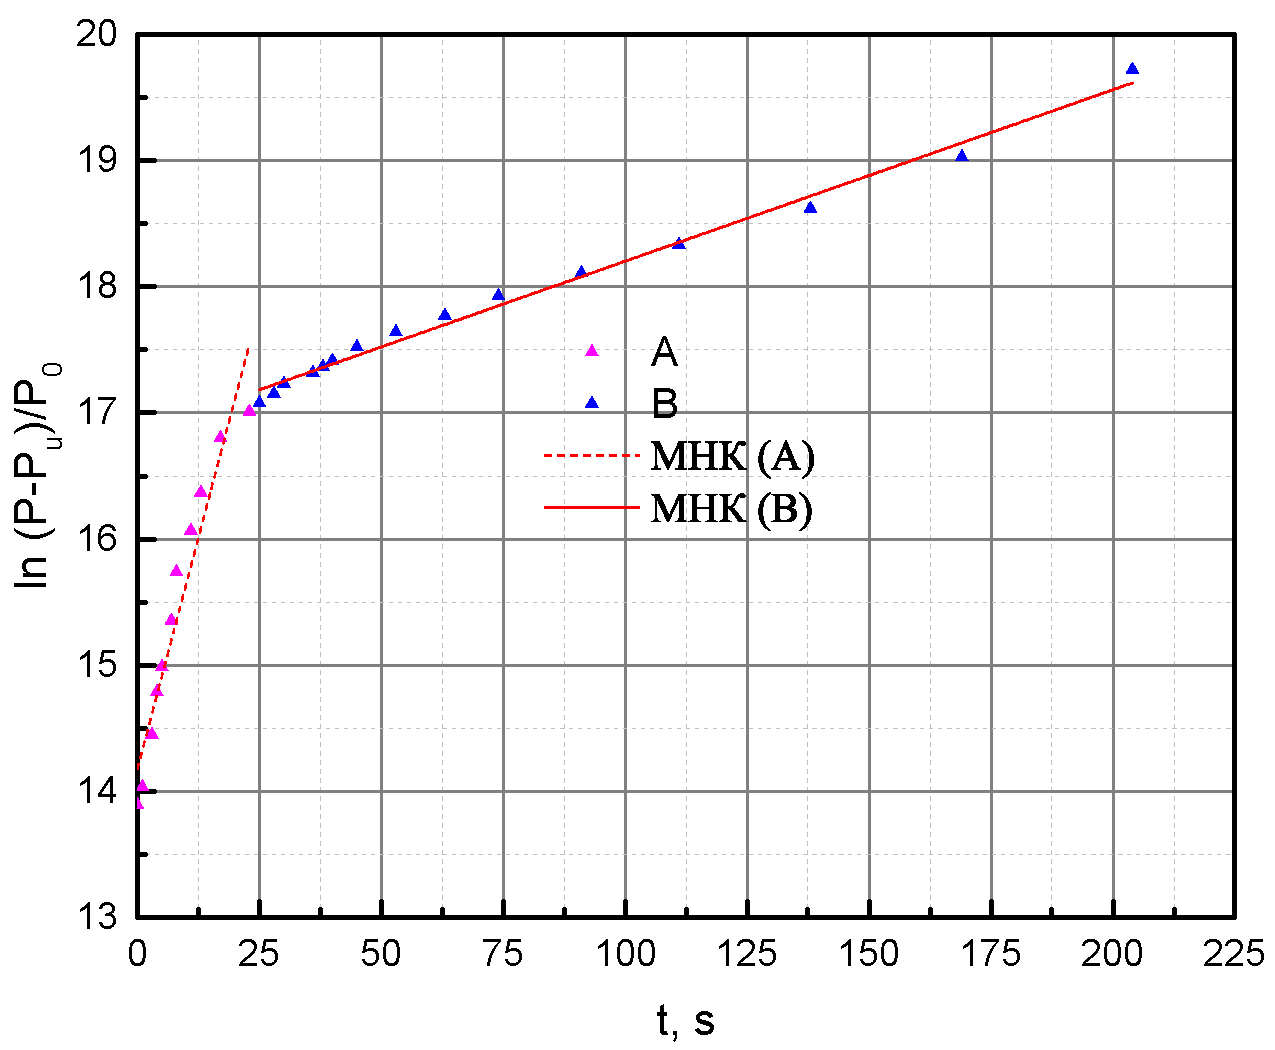
\includegraphics[scale=0.5]{Graph_upgrade.pdf}}
	\caption{Зависимость $\ln {(P-P_{pr})/P_0}$ от $t$.}
	\label{ris:Graph_upgrade}
\end{figure}

\floatsetup[table]{capposition=top}	
\begin{table}[H]
\caption{Результаты измерений.}
\label{table:results_upgrade}
\begin{tabular}{|c|c|c|}
\hline
$t$, с & $P$, 10$^{-6}$ торр & $\ln {(P-P_{pr})/P_0}$ \\ \hline
0      & 740              & 13,89                 \\ \hline
1      & 650              & 14,03                 \\ \hline
3      & 450              & 14,45                 \\ \hline
4      & 340              & 14,79                 \\ \hline
5      & 290              & 14,98                 \\ \hline
7      & 220              & 15,35                 \\ \hline
8      & 170              & 15,74                 \\ \hline
11     & 140              & 16,07                 \\ \hline
13     & 120              & 16,37                 \\ \hline
17     & 100              & 16,80                 \\ \hline
23     & 93               & 17,01                 \\ \hline
25     & 91               & 17,08                 \\ \hline
28     & 89               & 17,15                 \\ \hline
30     & 87               & 17,23                 \\ \hline
36     & 85               & 17,32                 \\ \hline
38     & 84               & 17,37                 \\ \hline
40     & 83               & 17,41                 \\ \hline
45     & 81               & 17,52                 \\ \hline
53     & 79               & 17,64                 \\ \hline
63     & 77               & 17,77                 \\ \hline
74     & 75               & 17,93                 \\ \hline
91     & 73               & 18,11                 \\ \hline
111    & 71               & 18,33                 \\ \hline
138    & 69               & 18,62                 \\ \hline
169    & 67               & 19,02                 \\ \hline
204    & 65               & 19,72                 \\ \hline
\end{tabular}
\end{table}

	Кривую, представленную на рис.~\ref{ris:Graph_upgrade}, методом наименьших квадратов аппроксимируем двумя прямыми "A" и "B" в компьютерной программе <<OriginPro>>. Наклоны прямых представлены в таблице~\ref{table:result_of_W/V}.
	
	
\floatsetup[table]{capposition=top}	
\begin{table}[H]
\caption{Результаты вычислений.}
\label{table:result_of_W/V}
\begin{tabular}{|c|c|c|c|c|}
\hline
$W/V$, с$^{-1}$ & $\sigma_{W/V}$, с$^{-1}$ & $W$, л/c & $\sigma_W$, л/с & $\varepsilon_W$, \% \\ \hline
0,198           & 0,008                    & 3,31     & 0,13            & 3,9                 \\ \hline
0,0140          & 0,0006                   & 0,23     & 0,01            & 4,3                 \\ \hline
\end{tabular}
\end{table}

	Значения высокого вакуума  торр в высоковакуумной части и низкого вакуума торр в форвакуумной части установки: $P_1 = 1,6 \cdot 10^{-4}$ и $P_2 = 1,9 \cdot 10^{-2}$. В нашем случае характерные параметры трубы и условия экспермиента -- $L = 70$ мм, $r = 0,9$ мм, $T = 293$ К, $\mu = 29$ г/моль. Тогда при численном расчете $W$ по формуле~(\ref{formula}) получим:
\begin{equation*}
	W = 0,25 \, \text{л/с}
\end{equation*}


\newpage
\section{Обсуждение результатов}
	Итак, в ходе данной лабораторной работы нам удалось получить высокий вакуум ($P = 6,3 \cdot 10^{-5}$ торр) с помощью диффузионного и форвакуумного насосов. Рассчитали скорость откачки насоса двумя независимыми способами: по улучшению вакуума и по скорости течения газа через трубу в условиях высокого вакуума. Результаты отличаются менее чем на 5\%, поэтому можно утверждать, что они совпадают в пределах погрешности. Стоит отметить, что построенный график (рис.~\ref{ris:Graph_upgrade}) оказался не сплошной прямой, как можно было предположить, а представим в виде двух прямых с сильно отличающимися углами наклона (более чем на 90\%. Естественно, что это связано с падением концентрации молекул, а это в свою очередь влияет на скорость откачки. Именно поэтому практический интерес представляет прямая "B".
	
	Вакуум необходим для получения тонких магнитных пленок. Важнейшей областью применения магнитных пленок является их использование для записи и хранения информации в запоминающих устройствах. Для увеличения плотности записи в магнитных пленках намагниченность ориентируют перпендикулярно плоскости пленок. Перпендикулярная ориентация намагниченности в тонких пленках энергетически невыгодна. Сильная перпендикулярная анизотропия в магнитных пленках возможна только при определенных условиях: толщина магнитного материала должна быть не выше критической и магнитный материал должен быть ограничен слоями некоторых тяжелых металлов (Pd, Pt, Ru). Именно граничные слои наводят перпендикулярную анизотропию во всей магнитной пленке. Напыление магнитного материала и тяжелых металлов, например, кобальта ($Co$) и ($Pd$) на кремниевую подложку ($SiO_2$) возможно только в сверхвысоком вакууме.
	
\section{Выводы}
\begin{enumerate}
\item
	Получили высокий вакуум: $P = 6,3 \cdot 10^{-5}$ торр.

\item
	По улучшению вакуума определили скорость откачки насоса: \\$W = (0,23 \pm 0,01)$ л/с.
	
\item
	По скорости течения газа в трубе в высоком вакууме определили скорость откачки насоса:  $W = 0,25$ л/с.


\end{enumerate}









\end{document}
